\documentclass[10pt]{article}

\usepackage[margin=0.75in]{geometry}
\usepackage{amsmath,amsthm,amssymb}
\usepackage{xcolor}
\usepackage{cancel}
\usepackage{xcolor}
\usepackage{tikz}
\usepackage{pgfplots}
\usepackage{physics}
\usepackage{minted}
\usepackage{pythonhighlight}
\usepackage{pdfpages}
\usepackage[inline]{enumitem}
\usepackage[breakable]{tcolorbox}

\theoremstyle{definition}
\newtheorem{problem}{Problem}
\newtheorem{soln}{Solution}

\pgfplotsset{compat=newest}
\usetikzlibrary{patterns}

\definecolor{incolor}{HTML}{303F9F}
\definecolor{outcolor}{HTML}{D84315}
\definecolor{cellborder}{HTML}{CFCFCF}
\definecolor{cellbackground}{HTML}{F7F7F7}

\tikzset
{%
  axes/.style={thick,-latex},
  cylinder/.style={right color=blue!80,left color=white,fill opacity=0.7},
  paraboloid back/.style={left color=magenta!80,fill opacity=0.4},
  paraboloid front/.style={left color=white, right color=magenta!80,fill opacity=0.4},
}

\makeatletter
\newcommand{\boxspacing}{\kern\kvtcb@left@rule\kern\kvtcb@boxsep}
\makeatother
\newcommand{\prompt}[4]{
    \ttfamily\llap{{\color{#2}[#3]:\hspace{3pt}#4}}\vspace{-\baselineskip}
}


\NewDocumentCommand{\evalat}{sO{\big}mm}{%
  \IfBooleanTF{#1}
   {\mleft. #3 \mright|_{#4}}
   {#3#2|_{#4}}%
}

\newcommand\nnfootnote[1]{%
  \begingroup
  \renewcommand\thefootnote{}\footnote{#1}%
  \addtocounter{footnote}{-1}%
  \endgroup
}


\title{Calculus II: Assignment 4}
\author{Jeremy Favro}
\date{\today}

% DOC BEGIN

\begin{document}

\maketitle

\noindent Consider the region below the curve $y = \frac{1}{x}$ and above the $x$-axis for $1 \leq x < \infty$.
% PROBLEM 1
\begin{problem}
Compute each of the following as best you can using SageMath.
\end{problem}
\begin{soln}
    $$\int_{1}^{\infty} \frac{1}{x} \,dx$$
    \begin{tcolorbox}[breakable, size=fbox, boxrule=1pt, pad at break*=1mm,colback=cellbackground, colframe=cellborder]
        \prompt{In}{incolor}{1}{\boxspacing}
        \begin{minted}[breaklines, autogobble]{sage}
            clear_vars()
            from sage.symbolic.integration.integral import definite_integral
            
            x = var('x')
            n = var('n')
            
            f = 1/x
            
            assume(n-1>0)
            
            definite_integral(f, x, 1, oo)
        \end{minted}
    \end{tcolorbox}
    \begin{tcolorbox}[breakable, size=fbox, boxrule=.5pt, pad at break*=1mm, opacityfill=0]
        \prompt{Out}{outcolor}{1}{\boxspacing}
        \begin{minted}[breaklines, autogobble]{sage}
            ValueError: Integral is divergent.
        \end{minted}
    \end{tcolorbox}

    $$\sum_{n = 1}^{\infty} \frac{1}{x}$$
    \begin{tcolorbox}[breakable, size=fbox, boxrule=1pt, pad at break*=1mm,colback=cellbackground, colframe=cellborder]
        \prompt{In}{incolor}{2}{\boxspacing}
        \begin{minted}[breaklines, autogobble]{sage}
            clear_vars()
            from sage.symbolic.integration.integral import definite_integral
            
            x = var('x')
            n = var('n')
            
            f = 1/x
            
            sum(f, x, 1, oo)
        \end{minted}
    \end{tcolorbox}
    \begin{tcolorbox}[breakable, size=fbox, boxrule=.5pt, pad at break*=1mm, opacityfill=0]
        \prompt{Out}{outcolor}{2}{\boxspacing}
        \begin{minted}[breaklines, autogobble]{sage}
            ValueError: Sum is divergent.
        \end{minted}
    \end{tcolorbox}

    \newpage

    $$\int_{1}^{\infty} \frac{1}{x^2} \,dx$$
    \begin{tcolorbox}[breakable, size=fbox, boxrule=1pt, pad at break*=1mm,colback=cellbackground, colframe=cellborder]
        \prompt{In}{incolor}{3}{\boxspacing}
        \begin{minted}[breaklines, autogobble]{sage}
            clear_vars()
            from sage.symbolic.integration.integral import definite_integral
            
            x = var('x')
            n = var('n')
            
            f = 1/x^2
            
            assume(n-1>0)
            
            limit(definite_integral(f, x, 1, n), n=oo)
        \end{minted}
    \end{tcolorbox}
    \begin{tcolorbox}[breakable, size=fbox, boxrule=.5pt, pad at break*=1mm, opacityfill=0]
        \prompt{Out}{outcolor}{3}{\boxspacing}
        \begin{minted}[breaklines, autogobble]{sage}
            1
        \end{minted}
    \end{tcolorbox}

    $$\sum_{n = 1}^{\infty} \frac{1}{x^2}$$
    \begin{tcolorbox}[breakable, size=fbox, boxrule=1pt, pad at break*=1mm,colback=cellbackground, colframe=cellborder]
        \prompt{In}{incolor}{4}{\boxspacing}
        \begin{minted}[breaklines, autogobble]{sage}
            clear_vars()
            from sage.symbolic.integration.integral import definite_integral
            
            x = var('x')
            n = var('n')
            
            f = 1/x^2
            
            sum(f, x, 1, oo) # Not quite sure why but this gives a nicer output than using a limit
        \end{minted}
    \end{tcolorbox}
    \begin{tcolorbox}[breakable, size=fbox, boxrule=.5pt, pad at break*=1mm, opacityfill=0]
        \prompt{Out}{outcolor}{4}{\boxspacing}
        \begin{minted}[breaklines, autogobble]{sage}
            1/6*pi^2
        \end{minted}
    \end{tcolorbox}

\end{soln}

% PROBLEM 2
\begin{problem}
Explain why the sum $\sum_{n = 1}^{\infty} \frac{1}{x}$ is what it is because the integral $\int_{1}^{\infty} \frac{1}{x} \,dx $ is what it is.
\end{problem}
\begin{soln} ~\\
    \begin{center}
        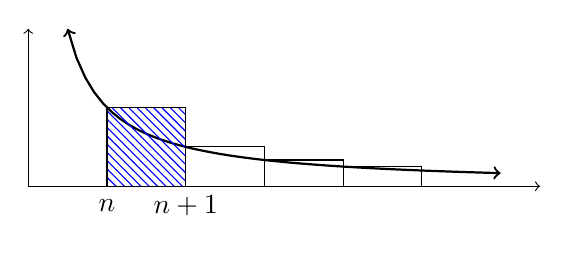
\begin{tikzpicture}
            \draw[<->] (0,2) -- (0,0) -- (6.5,0);
            \draw[thick, <->] plot[domain=.5:6,samples=50] (\x,{1/\x});
            \foreach \i/\j in {1/1,2/2,3/3,4/n} {
                    \draw (\i+1,0) rectangle (\i,{1/\i});
                    % \draw[dashed] (0,{1/\i}) -- ++ (\i-1,0) node[at start,left] {$\frac{1}{\j}$};
                }

            \node at (1,-0.25) {$n$};
            \node at (2,-0.25) {$n+1$};

            \draw[pattern=north west lines, pattern color=blue] (1+1,0) rectangle (1,{1});

        \end{tikzpicture}
    \end{center}

    \noindent Looking at the above figure and focusing on a single rectangle, starting at $n$ and ending at $n+1$ we can see that

    $$\int_{n}^{n+1} \frac{1}{x} \,dx <\footnote{I think this could also be called less than or equal as they'd approach each other as $\frac{d}{dx}\frac{1}{x}\to 0$, but I'm not sure if it's proper to say that} \frac{1}{n}$$

    \noindent Which can be extended to the whole curve

    $$\sum_{n = 1}^{\infty} \left[\int_{n}^{n+1} \frac{1}{x} \,dx\right] < \sum_{n = 1}^{\infty}\frac{1}{n}$$
    $$\int_{1}^{\infty} \frac{1}{x} \,dx < \sum_{n = 1}^{\infty}\frac{1}{n}$$

    \noindent We can then see that the area under the curve given by the integral is less than the area given by the sum. Computing the integral

    \begin{align*}
         & = \int_{1}^{\infty} \frac{1}{x} \,dx                 \\
         & = \lim_{r \to \infty}  \int_{1}^{r} \frac{1}{x} \,dx \\
         & = \lim_{r \to \infty}  \evaluated{\ln x}_{1}^{r}     \\
         & = \lim_{r \to \infty}  \ln(r)-0                      \\
         & = +\infty                                            \\
    \end{align*}

    \noindent We can now see that because the integral is infinite (Sage says divergent, from my understanding of it in the textbook that's basically the same thing), and the sum is greater than the integral, the sum must also be infinite.
\end{soln}

% PROBLEM 3
\begin{problem}
Explain why the sum $\sum_{n = 1}^{\infty} \frac{1}{n^2}$ has a finite value because the integral $\int_{1}^{\infty} \frac{1}{x^2} \,dx $ has a finite value.
\end{problem}
\begin{soln} ~\\
    \begin{center}
        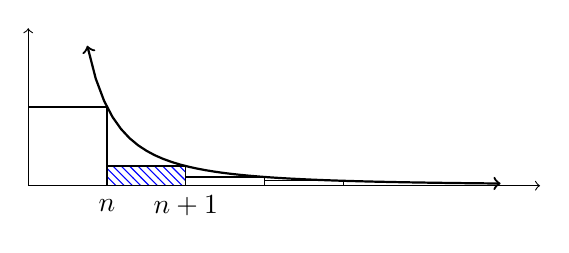
\begin{tikzpicture}
            \draw[<->] (0,2) -- (0,0) -- (6.5,0);
            \draw[thick, <->] plot[domain=0.75:6,samples=50] (\x,{1/\x^2});
            \foreach \i/\j in {1/1,2/2,3/3,4/n} {
                    \draw (\i-1,0) rectangle (\i,{1/\i^2});
                    % \draw[dashed] (0,{1/\i}) -- ++ (\i-1,0) node[at start,left] {$\frac{1}{\j}$};
                }

            \node at (1,-0.25) {$n$};
            \node at (2,-0.25) {$n+1$};

            \draw[pattern=north west lines, pattern color=blue] (1,0) rectangle (2,{0.25});
        \end{tikzpicture}
    \end{center}
    \noindent We can employ basically the same trick for this problem as the last, we just need to find a sum that gives the rectangles shown in the above figure and can somehow be equated to the given sum.
    The rectangles shown in the figure have an area of $\frac{1}{(n+1)^2}$, meaning that the sum $\sum_{n = 1}^{k} \frac{1}{(n+1)^2}$ can be used to obtain them.
    $$\sum_{n = 1}^{k} \frac{1}{n^2} = \frac{1}{1^2}+\frac{1}{2^2}+\frac{1}{3^2}+\dots+\frac{1}{k^2}$$
    $$\sum_{n = 1}^{k} \frac{1}{(n+1)^2} = \frac{1}{2^2}+\frac{1}{3^2}+\dots+\frac{1}{(k+1)^2}$$

    \noindent So,
    $$\sum_{n = 1}^{k} \frac{1}{(n+1)^2} = \sum_{n = 1}^{k} \frac{1}{n^2}-1$$

    \noindent Using the graph to identify that the integral will always be greater\footnotemark[1] than the sum

    $$\int_{n}^{n+1} \frac{1}{x^2} \,dx > \frac{1}{(n+1)^2}  $$
    $$\sum_{n = 1}^{\infty}\int_{n}^{n+1} \frac{1}{x^2} \,dx > \sum_{n = 1}^{\infty} \frac{1}{(n+1)^2} $$
    $$\int_{1}^{\infty} \frac{1}{x^2} \,dx > \sum_{n = 1}^{\infty} \frac{1}{(n+1)^2} $$

    \noindent But we are looking to explain the finiteness of $\sum_{n = 1}^{n} \frac{1}{n^2}$, not $\sum_{n = 1}^{n} \frac{1}{(n+1)^2}$. So we need to use the equality determined earlier

    $$\int_{1}^{\infty} \frac{1}{x^2} \,dx > \sum_{n = 1}^{\infty} \frac{1}{(n+1)^2}= \sum_{n = 1}^{\infty} \frac{1}{n^2}-1$$
    $$\int_{1}^{\infty} \frac{1}{x^2} \,dx + 1 > \sum_{n = 1}^{\infty} \frac{1}{n^2}$$

    \noindent We can then see that the area under the curve given by the integral is greater than the area given by the sum. Computing the integral

    \begin{align*}
         & = \int_{1}^{\infty} \frac{1}{x^2} \,dx                  \\
         & = \lim_{r \to \infty}  \int_{1}^{r} \frac{1}{x^2} \,dx  \\
         & = \lim_{r \to \infty}  \evaluated{-\frac{1}{x}}_{1}^{r} \\
         & = \lim_{r \to \infty}  0+\frac{1}{1}                    \\
         & = 1                                                     \\
    \end{align*}

    \noindent So,
    $$\sum_{n = 1}^{\infty} \frac{1}{n^2} < 2$$

    \noindent And the sum has an implicit lower bound of zero as it will never start adding negative terms, so, the sum must be finite and inbetween 0 and 2.
\end{soln}

% PROBLEM 4
\begin{problem}
Explain why the limit $\lim_{k \to \infty} \left[\sum_{n = 1}^{k} \frac{1}{n} - \ln(k+1)\right]$ exists and is between 0 and 1.
\end{problem}
\begin{soln} ~\\
    \begin{center}
        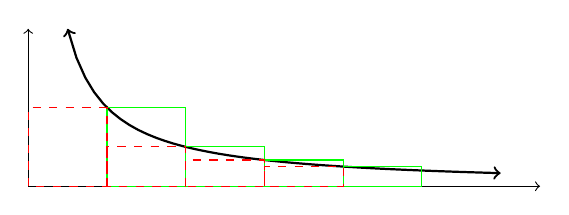
\begin{tikzpicture}
            \draw[<->] (0,2) -- (0,0) -- (6.5,0);
            \draw[thick, <->] plot[domain=.5:6,samples=50] (\x,{1/\x});
            \foreach \i/\j in {1/1,2/2,3/3,4/n} {
                    \draw[color=green] (\i+1,0) rectangle (\i,{1/\i});
                    \draw[color=red, dashed] (\i-1,0) rectangle (\i,{1/\i});
                }
        \end{tikzpicture}
    \end{center}

    \noindent Observing the limit and the figure it becomes relatively clear to see that the limit is just the overestimate created by the rectangles of summation. To begin with defining the bounds for
    that overestimate, it helps to slightly rejig the limit.

    \begin{align*}
         & = \lim_{k \to \infty} \left[\sum_{n = 1}^{k} \frac{1}{n} - \ln(k+1)\right]                                         \\
         & = \lim_{k \to \infty} \left[\sum_{n = 1}^{k} \frac{1}{n} - \int_{1}^{k+1} \frac{1}{x} \,dx \right]                 \\
         & = \lim_{k \to \infty} \left[\sum_{n = 1}^{k} \frac{1}{n} - \sum_{n = 1}^{k}\int_{n}^{n+1} \frac{1}{x} \,dx \right] \\
         & = \lim_{k \to \infty} \left[\sum_{n = 1}^{k} \left(\frac{1}{n} - \int_{n}^{n+1} \frac{1}{x} \,dx \right)\right]    \\
    \end{align*}

    \noindent We know that for a function that is decreasing on an interval, the \textcolor{red}{Right Riemann Sum} understimates the area under the curve, and the \textcolor{green}{Left Riemann Sum} overestimates, creating bounds for the integral
    $$\frac{1}{n+1}\leq\int_{n}^{n+1} \frac{1}{x} \,dx\leq \frac{1}{n}$$.

    \noindent The bounds for the integral can then be used to demonstrate that
    $$0 < \sum_{n = 1}^{k}\left[ \frac{1}{n} - \int_{n}^{n+1} \frac{1}{x} \,dx\right]$$
    \noindent which establishes our lower bound.
    ~\\
    ~\\
    \noindent Then, establishing an upper bound uses a similar trick where we show that for any $n$, the area between the RRS and LRS rectangles ($LRS_n - RRS_n$) is greater than
    the integral for that interval.
    $$\sum_{n = 1}^{k}\left[ \frac{1}{n} - \int_{n}^{n+1} \frac{1}{x} \,dx\right] < \sum_{n = 1}^{k}\left[\frac{1}{n} - \frac{1}{n+1}\right]$$

    \noindent Then simplifying and taking the limit of all three sides to determine the actual bounds
    $$0 < \sum_{n = 1}^{k}\left[ \frac{1}{n} - \int_{n}^{n+1} \frac{1}{x} \,dx\right] < \frac{k}{k+1}$$
    $$\lim_{k \to \infty}0 < \lim_{k \to \infty}\sum_{n = 1}^{k}\left[ \frac{1}{n} - \int_{n}^{n+1} \frac{1}{x} \,dx\right] < \lim_{k \to \infty}\frac{k}{k+1}$$
    $$0 < \lim_{k \to \infty}\sum_{n = 1}^{k}\left[ \frac{1}{n} - \int_{n}^{n+1} \frac{1}{x} \,dx\right] < 1$$
    $$0 < \lim_{k \to \infty} \left[\sum_{n = 1}^{k} \frac{1}{n} - \ln(k+1)\right] < 1$$
\end{soln}

% PROBLEM 4
\begin{problem}
Use SageMath to (approximately) evaluate $\lim_{k \to \infty} \left[\sum_{n = 1}^{k} \frac{1}{n} - \ln(k+1)\right]$ as best you can.
\end{problem}
\begin{soln} ~\\
    \begin{tcolorbox}[breakable, size=fbox, boxrule=1pt, pad at break*=1mm,colback=cellbackground, colframe=cellborder]
        \prompt{In}{incolor}{1}{\boxspacing}
        \begin{minted}[breaklines, autogobble]{sage}
                clear_vars()
                from sage.symbolic.integration.integral import definite_integral
                
                k = var('k')
                x = var('x')
                n = var('n')
                
                N(limit((sum((1/n), n, 1, k))-ln(k+1), k=9999)) # As k -> infty this should get better and better, but Sage doesn't like that so I've just put a big number
            \end{minted}
    \end{tcolorbox}
    \begin{tcolorbox}[breakable, size=fbox, boxrule=.5pt, pad at break*=1mm, opacityfill=0]
        \prompt{Out}{outcolor}{1}{\boxspacing}
        \begin{minted}[breaklines, autogobble]{sage}
                0.577165664068199
            \end{minted}
    \end{tcolorbox}
\end{soln}


\end{document}